\documentclass[preprint,12pt,aps,pra,showkeys,amsmath,amssymb,superscriptaddress,floatfix]{revtex4-2}
\usepackage[T1]{fontenc}
\usepackage[utf8]{inputenc}
\usepackage{amsmath,amssymb,amsthm,mathtools,mathrsfs}
\usepackage{microtype,booktabs,enumitem}
\usepackage{xcolor,tikz,etoolbox}
\usepackage[skins,breakable]{tcolorbox}
\usepackage{needspace}
% Keep diagram geometry independent of REVTeX preprint body spacing.
\AtBeginEnvironment{tikzpicture}{\linespread{1}\selectfont}
\usetikzlibrary{arrows.meta,positioning,calc,fit,decorations.pathreplacing}
\usepackage{graphicx}
\usepackage{hyperref}

\definecolor{MMBlue}{RGB}{0,82,155}
\definecolor{MMOrange}{RGB}{200,80,0}
\tikzset{
 mmnode/.style={draw=MMBlue,rounded corners=2pt,fill=MMBlue!4,align=left,execute at begin node={\raggedright},text width=5cm,font=\fontsize{10}{12}\selectfont,inner sep=6pt},
 mmimport/.style={mmnode,draw=black!65,fill=black!4},
 mmcandidate/.style={mmnode,draw=MMOrange,dashed,fill=MMOrange!5},
 mmrejected/.style={mmnode,draw=black,densely dotted,fill=black!8},
 mmproof/.style={->,thick,MMBlue},
 mmflow/.style={->,semithick,black!70},
 mmrepair/.style={->,dashed,thick,MMOrange},
 mmcandidatearrow/.style={->,dashed,semithick,MMOrange},
 mmnote/.style={font=\scriptsize,fill=white,inner sep=2pt,align=center}}

\usepackage[section]{placeins}
\setlength{\emergencystretch}{3em}
\setlist{itemsep=3pt,topsep=4pt}
\newtheorem{theorem}{Theorem}[section]
\newtheorem{proposition}[theorem]{Proposition}
\newtheorem{lemma}[theorem]{Lemma}
\newtheorem{corollary}[theorem]{Corollary}
\theoremstyle{definition}
\newtheorem{definition}[theorem]{Definition}
\newtheorem{example}[theorem]{Example}
\theoremstyle{remark}
\newtheorem{remark}[theorem]{Remark}
% Avoid isolated statement headings and single-line paragraph fragments.
\BeforeBeginEnvironment{theorem}{\Needspace{6\baselineskip}}
\BeforeBeginEnvironment{definition}{\Needspace{5\baselineskip}}
\BeforeBeginEnvironment{proposition}{\Needspace{5\baselineskip}}
\BeforeBeginEnvironment{lemma}{\Needspace{5\baselineskip}}
\BeforeBeginEnvironment{corollary}{\Needspace{5\baselineskip}}
\clubpenalty=5000
\widowpenalty=5000
\newcommand{\R}{\mathbb R}\newcommand{\Z}{\mathbb Z}\newcommand{\N}{\mathbb N}
\newcommand{\Pa}{\operatorname{Pa}}\newcommand{\Desc}{\operatorname{Desc}}
\newcommand{\cl}{\operatorname{cl}}\newcommand{\cost}{\operatorname{cost}}
\newcommand{\status}{\operatorname{status}}
% Faculty cards: a visual rail groups the five faculties within one agent.
% The rail has no arrowhead and does not represent a proof dependency.
\newcommand{\mmfacultybadge}[1]{%
 \node[circle,draw=MMBlue,line width=1pt,fill=white,
 minimum size=7mm,inner sep=0pt,font=\sffamily\small\bfseries,text=MMBlue]
 at ([xshift=15pt,yshift=-15pt]frame.north west) {#1};}
\newcommand{\mmfacultyrail}{%
 \draw[MMBlue!80,line width=1pt]
 ([xshift=15pt,yshift=2pt]frame.north west)--
 ([xshift=15pt,yshift=-2pt]frame.south west);}
\newtcolorbox{mmfacultybox}[2]{enhanced,breakable,
 colback=MMBlue!4,colframe=MMBlue!4,boxrule=0pt,arc=3pt,
 left=39pt,right=9pt,top=4pt,bottom=4pt,
 before skip=2pt,after skip=2pt,
 fontupper=\small\linespread{1.1}\selectfont,
 overlay unbroken={\mmfacultyrail\mmfacultybadge{#1}},
 overlay first={\mmfacultyrail\mmfacultybadge{#1}},
 overlay middle={\mmfacultyrail},overlay last={\mmfacultyrail}}
\newcommand{\mmfaculty}[3]{%
 \begin{mmfacultybox}{#1}{#2}
 {\sffamily\bfseries\color{MMBlue}#2}\par\smallskip #3
 \end{mmfacultybox}}
\newcommand{\agent}[9]{%
 \Needspace{8\baselineskip}
 \subsubsection{#1}
 \noindent\textbf{Object.} #2\par
 \noindent\textbf{Role.} #3\par\smallskip
 \mmfaculty{E}{Ego}{#4}
 \mmfaculty{M}{Memory}{#5}
 \mmfaculty{I}{Intellect}{#6}
 \mmfaculty{S}{Sense}{#7}
 \mmfaculty{A}{Action}{#8}
 \smallskip\noindent #9\par}

\usepackage{longtable,array,calc}
\providecommand{\tightlist}{\setlength{\itemsep}{2pt}\setlength{\parskip}{0pt}}
\makeatletter
\def\frontmatter@abstract@produce{\par\addvspace{\frontmatter@preabstractspace}%
\begingroup\prep@absbox\unvbox\absbox\post@absbox\endgroup
\addvspace{\frontmatter@postabstractspace}}
\makeatother
\newcommand{\field}[2]{\par\smallskip\noindent\textbf{#1.} #2\par}
\setlength{\emergencystretch}{5em}
\AtBeginEnvironment{verbatim}{\small\linespread{1.0}\selectfont}


\hypersetup{colorlinks=true,linkcolor=MMBlue,urlcolor=MMBlue,pdfauthor={Dibakar Sigdel}}

\begin{document}

\title{Energy Decay and Uniqueness for the Heat Equation\\[4pt]\large An End-to-End Meta-Math Walkthrough}

\author{Dibakar Sigdel}

\affiliation{Mindverse Computing LLC, Lynnwood, WA 98087, USA}

\date{October 2026}

\begin{abstract}

The squared \(L^2\) difference is an energy. Its derivative is the
negative of a nonnegative gradient integral, so identical initial states
cannot separate. The report presents the target theorem, declared
imports, a dependency graph, five-faculty node contracts, a continuous
proof, a worked example, and a hypothesis-repair audit. It is an
authored mathematical exposition, not a deployed-agent transcript or a
formal proof-assistant certificate.

\end{abstract}\maketitle\linespread{1.12}\selectfont

\noindent\textbf{PDE-03 / Partial Differential Equations / Report v1}

\section{Target and import contract}

\begin{theorem}

Let \(\Omega\subset\mathbb R^d\) be bounded with \(C^1\) boundary,
\(T>0\), and \(\kappa>0\). Suppose real \(u,v\) have continuous spatial
derivatives through order two and time derivative through order one on
\(\overline\Omega\times[0,T]\), solve
\(u_t-\kappa\Delta u=v_t-\kappa\Delta v\), and agree on the lateral
boundary. Prove
\(\|u(\cdot,t)-v(\cdot,t)\|_2^2+2\kappa\int_0^t\|\nabla(u-v)(\cdot,s)\|_2^2ds=\|u(\cdot,0)-v(\cdot,0)\|_2^2\).
In particular equal initial data imply \(u=v\).

\end{theorem}

\subsection{Foundations and permitted imports}

Use differentiation under an integral for continuous derivatives on the
compact cylinder, Green's integration-by-parts identity on the \(C^1\)
domain for the stated regularity, and the fundamental theorem of
calculus. The difference \(w=u-v\) solves a homogeneous heat equation
with zero boundary values. No existence result or unbounded-domain
uniqueness is asserted here.

\clearpage\section{Node interaction workflow}

\begin{center}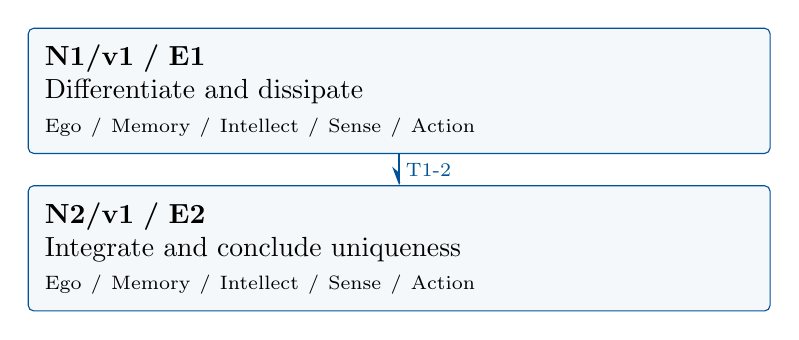
\begin{tikzpicture}[>=Stealth,x=1cm,y=1cm]

\node[mmnode,text width=9cm,minimum height=1.25cm] (N1) at (0,0.0) {\textbf{N1/v1 / E1}\\Differentiate and dissipate\\{\scriptsize Ego / Memory / Intellect / Sense / Action}};

\node[mmnode,text width=9cm,minimum height=1.25cm] (N2) at (0,-2.0) {\textbf{N2/v1 / E2}\\Integrate and conclude uniqueness\\{\scriptsize Ego / Memory / Intellect / Sense / Action}};

\draw[mmproof] (N1.south) -- node[mmnote,right] {T1-2} (N2.north);

\end{tikzpicture}\end{center}

Each box is one mathematical agent containing all five faculties. Blue
arrows carry the versioned exports listed below. The layout gives a
reading order; only drawn arrows assert dependencies. Diagnostic repair
is separate from the proof DAG.

\subsection{Versioned evidence-transfer ledger}

\begingroup\small\linespread{1.05}\selectfont

\Needspace{5\baselineskip}\field{T1-2: N1/E1/v1 to N2}{\(E(t)=\int_\Omega w^2\) satisfies
\(E'(t)=-2\kappa\int_\Omega|\nabla w|^2\).}

\field{Receiving activity}{N2.1}

\field{Compatibility}{E1/v1 and nonnegativity of both energy and dissipation. Check: An
integral norm equal to zero gives a.e. equality first; continuity
supplies equality at every interior point and the boundary data cover
the boundary.}

\endgroup

\clearpage\section{Agent roles and five-faculty activities}\begingroup\small\linespread{1.05}\selectfont\setlist{itemsep=1pt,topsep=2pt}

\subsection{N1/v1: Differentiate and dissipate}

\field{Object and role}{Multiply by the solution difference and transfer one spatial derivative
by Green's formula. \textbf{Local obligation:} \(E(t)=\int_\Omega w^2\)
satisfies \(E'(t)=-2\kappa\int_\Omega|\nabla w|^2\).}

\field{Inputs}{\(w=u-v\), \(w_t=\kappa\Delta w\), and \(w|_{\partial\Omega}=0\).}

\mmfaculty{E}{Ego}{Publish E1/v1 only after establishing this obligation:
\(E(t)=\int_\Omega w^2\) satisfies
\(E'(t)=-2\kappa\int_\Omega|\nabla w|^2\).}

\mmfaculty{M}{Memory}{\(w=u-v\), \(w_t=\kappa\Delta w\), and \(w|_{\partial\Omega}=0\). Retain
the stated assumptions and import versions.}

\mmfaculty{I}{Intellect}{Multiply by the solution difference and transfer one spatial derivative
by Green's formula.}

\mmfaculty{S}{Sense}{The boundary term vanishes because \(w=0\), not because its normal
derivative is assumed zero.}

\mmfaculty{A}{Action}{Carry out activities N1.1--N1.2 below, retaining each calculation and
construction as evidence.}

\smallskip\noindent\textbf{Numbered mathematical activities}

\begin{enumerate}[label=N1.\arabic*,leftmargin=3.4em]

\item The regularity and compactness allow
\(E'(t)=2\int_\Omega w w_t=2\kappa\int_\Omega w\Delta w\).

\item Green's identity gives
\(\int_\Omega w\Delta w=\int_{\partial\Omega}w\partial_\nu w-\int_\Omega|\nabla w|^2\).
The boundary value of \(w\) is zero, so the boundary integral vanishes.
This proves the exact energy derivative.

\end{enumerate}

\field{Export E1/v1}{\(E(t)=\int_\Omega w^2\) satisfies
\(E'(t)=-2\kappa\int_\Omega|\nabla w|^2\).}

\field{Acceptance gate}{The boundary term vanishes because \(w=0\), not because its normal
derivative is assumed zero.}

\field{Targeted repair}{If the boundary term is simply omitted, write it explicitly and use the
equality of boundary data to make the difference vanish there. Withhold
this export and recheck its descendants after a versioned correction.}

\clearpage

\subsection{N2/v1: Integrate and conclude uniqueness}

\field{Object and role}{Integrate the identity from zero to \(t\), then use continuity to
upgrade an \(L^2\) zero to pointwise equality. \textbf{Local
obligation:} The stated energy identity holds, and equal initial data
give equality of the two classical solutions.}

\field{Inputs}{E1/v1 and nonnegativity of both energy and dissipation. Incoming proof
exports: E1/v1 at N2.1.}

\mmfaculty{E}{Ego}{Publish E2/v1 only after establishing this obligation: The stated energy
identity holds, and equal initial data give equality of the two
classical solutions.}

\mmfaculty{M}{Memory}{E1/v1 and nonnegativity of both energy and dissipation. Incoming proof
exports: E1/v1 at N2.1. Retain the stated assumptions and import
versions.}

\mmfaculty{I}{Intellect}{Integrate the identity from zero to \(t\), then use continuity to
upgrade an \(L^2\) zero to pointwise equality.}

\mmfaculty{S}{Sense}{An integral norm equal to zero gives a.e. equality first; continuity
supplies equality at every interior point and the boundary data cover
the boundary.}

\mmfaculty{A}{Action}{Carry out activities N2.1--N2.2 below, retaining each calculation and
construction as evidence.}

\smallskip\noindent\textbf{Numbered mathematical activities}

\begin{enumerate}[label=N2.\arabic*,leftmargin=3.4em]

\item Integrating E1 yields
\(E(t)+2\kappa\int_0^t\int_\Omega|\nabla w(x,s)|^2\,dx\,ds=E(0)\). This
proves the claimed stability identity and \(E(t)\le E(0)\).

\item If the initial data agree, \(E(0)=0\). Nonnegativity forces \(E(t)=0\)
for each \(t\). Were continuous \(w\) nonzero at an interior point, it
would be bounded away from zero on a small ball, making the integral
positive. Thus \(w=0\) inside, and it is zero on the boundary by
assumption.

\end{enumerate}

\field{Export E2/v1}{The stated energy identity holds, and equal initial data give equality
of the two classical solutions.}

\field{Acceptance gate}{An integral norm equal to zero gives a.e. equality first; continuity
supplies equality at every interior point and the boundary data cover
the boundary.}

\field{Targeted repair}{If equality almost everywhere is treated as pointwise without
regularity, use continuity explicitly or state uniqueness only in the
appropriate equivalence class. Withhold this export and recheck its
descendants after a versioned correction.}

\endgroup\clearpage\section{Continuous mathematical proof}\label{sec:proof}

\subsection{N1 --- Differentiate and
dissipate}\label{n1-differentiate-and-dissipate}

\begin{enumerate}
\def\labelenumi{\arabic{enumi}.}
\item
  \textbf{N1.1.} The regularity and compactness allow
  \(E'(t)=2\int_\Omega w w_t=2\kappa\int_\Omega w\Delta w\).
\item
  \textbf{N1.2.} Green's identity gives
  \(\int_\Omega w\Delta w=\int_{\partial\Omega}w\partial_\nu w-\int_\Omega|\nabla w|^2\).
  The boundary value of \(w\) is zero, so the boundary integral
  vanishes. This proves the exact energy derivative.
\end{enumerate}

\subsection{N2 --- Integrate and conclude
uniqueness}\label{n2-integrate-and-conclude-uniqueness}

\begin{enumerate}
\def\labelenumi{\arabic{enumi}.}
\item
  \textbf{N2.1.} Integrating E1 yields
  \(E(t)+2\kappa\int_0^t\int_\Omega|\nabla w(x,s)|^2\,dx\,ds=E(0)\).
  This proves the claimed stability identity and \(E(t)\le E(0)\).
\item
  \textbf{N2.2.} If the initial data agree, \(E(0)=0\). Nonnegativity
  forces \(E(t)=0\) for each \(t\). Were continuous \(w\) nonzero at an
  interior point, it would be bounded away from zero on a small ball,
  making the integral positive. Thus \(w=0\) inside, and it is zero on
  the boundary by assumption.
\end{enumerate}

\hfill$\square$

\section{Worked orchestration}

On \((0,\pi)\) with \(\kappa=1\), take \(u(x,t)=e^{-t}\sin x\) and
\(v=0\). Then \(E(t)=(\pi/2)e^{-2t}\), and
\(\|u_x(\cdot,t)\|_2^2=(\pi/2)e^{-2t}\). Hence
\(E(t)+2\int_0^t\|u_x\|_2^2ds=\pi/2=E(0)\), checking the constants and
sign.

\subsection{Boundary and hypothesis audit}

If boundary equality is removed, \(u(x,t)=x\) and \(v=0\) on \((0,1)\)
are both time-independent heat solutions. Their difference has constant
energy \(1/3\), while its gradient integral is one. The missing boundary
flux equals one and exactly cancels the dissipation term; it cannot be
discarded.

\section{Illustrative failure and repair}

The following is an authored diagnostic scenario. Changed assumptions
define a new contract; they do not retroactively prove the original
statement.

\subsection{Rejected argument, diagnosis, and correction}
\textbf{Rejected N1 identity:} \(E'=-2\kappa\|\nabla w\|_2^2\) for
arbitrary boundary data. \textbf{Sense witness:} \(w=x\) on \((0,1)\).
\textbf{Repair:} retain the flux term in Green's identity and then use
the actual homogeneous difference boundary condition from §1. Recheck
the integrated identity and uniqueness. This repairs the proof of the
stated class, not a broader uniqueness claim.

\subsection{Publication and reuse}
The corrected export retains its explicit assumptions. A hypothetical
revision receives a new version, and each consuming activity is
rechecked; this scenario is not a recorded runtime event. \textbf{Next
direction:} Extend the energy method to weak parabolic solutions by
justifying time testing through approximation.

\par\medskip\begingroup\small\linespread{1.0}\selectfont\noindent\textbf{Provenance.} This authored proof is complete relative to its declared imports. Reuse
each export with its assumptions, proof, and version. The original
Markdown remains available for comparison.
\par\endgroup

\par\smallskip\begingroup\small\linespread{1.0}\selectfont\noindent\textbf{Further reading.} \href{https://math.stanford.edu/~lms/lecs-on-pde.pdf}{Leon Simon,
Lectures on PDE}, for elliptic, weak, and parabolic methods. Classical
calculus and the explicitly stated Hilbert-space imports are used below;
the displayed PDE arguments are developed in full.\par\endgroup

\end{document}
